\section{Auswertung}
\subsection{Versuchsaufbau}

\subsection{Kalibrierung}
Zunächst haben wir manuell eine Hallsonde in etwa im Zentrum des
Magnetspulenpaars positioniert, was dadurch erreicht wurde, dass die Position
der Sonde so lange verändert wurde, bis der maximale Wert des digital
ausgegebenen Messwerts der Hallsonde erreicht war. Da dann die Mitte des
Spulenpaars gefunden war, wurde die Hallsonde selbst im weiteren Experiment
nicht mehr bewegt. Die Messunsicherheit der Magnetfeldmessung liegt immer bei
der letzten angegebenen Nachkommastelle, also ist dieser Fehler hier $\pm
\SI{1}{\milli\tesla}$.

Da wir nun eine Möglichkeit hatten, Magnetfelder zu messen, wurde als Nächstes
das bei verschiedenen Stromstärken resultierende Magnetfeld untersucht. Dafür
wurde das Magnetfeld in \SI{1}{\ampere}-Schritten von 0 bis etwa 10,8 bzw.
\SI{-10,8}{\ampere} verändert und das jeweils
zugehörige Magnetfeld wurde als Messwert aufgenommen. Um den Einfluss von
Hysterese-Effekten zu untersuchen, wurde immer von kleinen zu großen
Stromstärken $I$ und anschließend wieder zurück von großen zu kleinen
Stromstärken gemessen. Dieses Vorgehen eignet sich, um die Größe der
Restmagnetisierung bei $I=0$ zu bestimmen. Die Messwerte können im Anhang unter
\ref{sec:messwerte} betrachtet werden. 

Wenn man nun diese Datenpunkte in einem Diagramm aufträgt, resultiert das in
\fref{hysterese} dargestellte Bild.

\begin{figure}[htb]
   \centering
   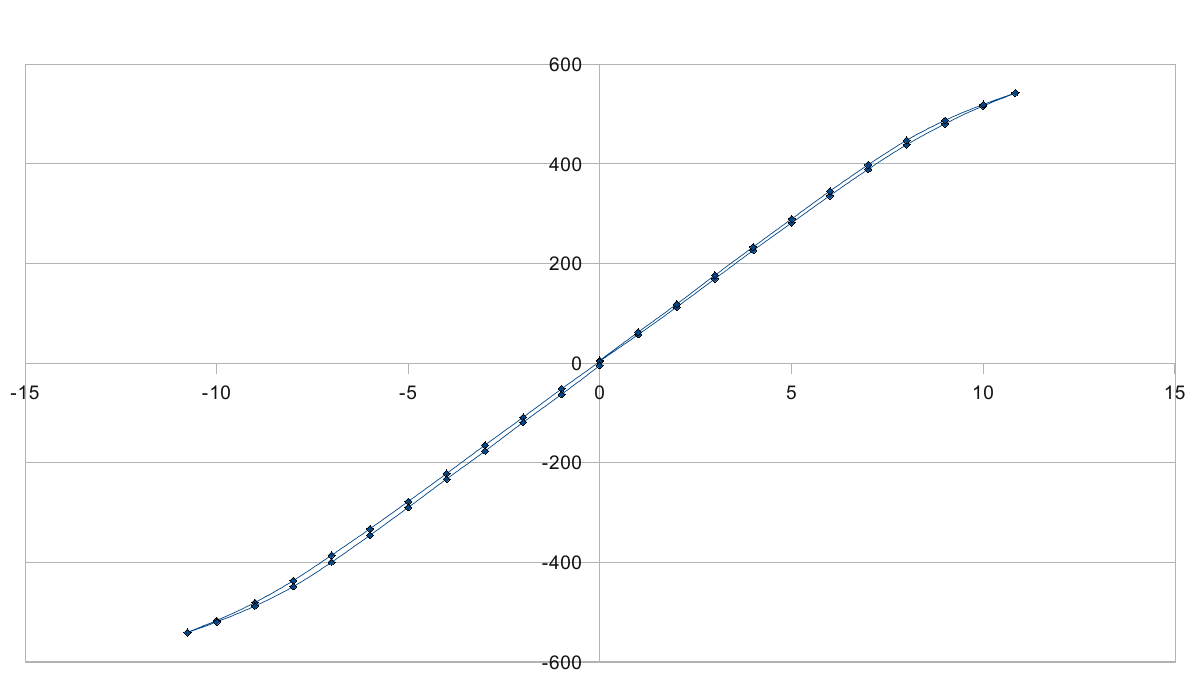
\includegraphics[width=1\columnwidth,keepaspectratio]{hysterese.png}
   \caption{Magnetfeldstärke in Abhängigkeit vom Erregerstrom $I$}
   \label{fig:hysterese}
\end{figure}

Wie man erkennen kann, ist nicht nur eine durchgehende Linie sichtbar, sondern
eine klassische Hysteresekurve mit zwei einzelnen Linien jeweils für $I<0$ und
für $I>0$ ist erkennbar. Allerdings verzichten wir im Weiteren auf eine genaue
Untersuchung der eingeschlossenen Fläche, sondern betrachten die Kurve als
jeweils eine Linie, und der Einfluss der Hysterese wird als Fehler dieser
Annahme betrachtet. Dies ist legitim, da die Abstände der Linien nie mehr als
ca. \SI{10}{\milli\tesla} beträgt, während die Messwerte schnell Bereiche von
100 bis \SI{500}{\milli\tesla} erreichen, sodass der Fehler dabei im
Prozentbereich liegt.

Fehlt hier noch ne Fitkurve oder so????

\subsection{Messung des elektrischen Widerstands des Kristalls bei
Raumtemperatur}
Um eine Vorstellung der Größenordnung der Widerstände, die zwischen den
einzelnen Kontakten unseres Halbleiterkristalls bestehen, zu erhalten, wurden
verschiedene Kombinationen von Kontakten daraufhin vermessen. Dabei haben wir
festgestellt, dass bei unserer Probe der Kontakt mit der Nummer fünf defekt
war, sodass nur die anderen im weiteren Versuch verwendet werden konnten. Die
einzelnen Messergebnisse der Widerstandsmessung können im Anhang unter
\ref{sec:messwerte} betrachtet werden. Wie man erkennen kann, liegen die
Werte, bei denen beide Messpunkte zum gleichen Kontakt gehörten, während die
eine Messspitze direkt an der Probe und die andere am Messpad anlag, im Bereich
um \SI{1}{\ohm}. Dies ist demnach die Größenordnung der Kabelwiderstände
inklusive der Kontaktwiderstände. Wenn nun der Widerstand zwischen
unterschiedlichen Kontaktpunkten gemessen wird, kann man feststellen, dass die 
Werte in einer ganz anderen Größenordnung von etwa 20 bis \SI{50}{\ohm} liegen.
Die Werte für die realen Widerstände liegen also im eben angegebenen Bereich,
wobei der Fehler durch die vorher beschriebenen Kontakt- und Kabelwiderstände
vernachlässigt werden kann, da diese wesentlich kleiner sind. Es muss aber
erwähnt werden, dass dieses Ergebnis nur bei Zimmertemperatur gültig ist, da
sich der Widerstand stark mit der Temperatur ändern wird.